%\documentclass[letter,6pt]{article}
\documentclass[A0,6pt]{article}

\usepackage[tagged]{accessibility}

\usepackage[margin=1cm,landscape]{geometry}

\usepackage{multicol}
\usepackage{tikz,lipsum,lmodern}
\usepackage[most]{tcolorbox}

\PassOptionsToPackage{hyphens}{url}
\usepackage[pdflang={en-US},pdftex, hidelinks]{hyperref}
\usepackage{booktabs,siunitx}
\usepackage{breakurl}

% \usepackage[table]{xcolor} 
\usepackage{fancyvrb}
\usepackage{listings}
\usepackage{xcolor}
\usepackage{tikz}
\usepackage{forest}
\usepackage{adjustbox}
\usetikzlibrary{arrows.meta,shadows}
\usepackage{array,multirow,graphicx}
\setcounter{tocdepth}{9}
\usepackage{enumitem} 
\usepackage{pifont}

%\providecommand{\tightlist}{%
%  \setlength{\itemsep}{0pt}\setlength{\parskip}{0pt}}

\newcommand{\TODO}[1]{\todo[inline]{#1}}

\newcommand{\RULE}{\hrule
\vspace{1pt}
\hrule height 1pt
}

\newcommand{\ngreen}{bottom color=green!20}
\newcommand{\ngrey}{bottom color=gray!20}
\newcommand{\nred}{bottom color=red!20}
\newcommand{\nwhite}{bottom color=white!20}

\newcommand{\Figure}[1]{Fig.~\ref{#1}}
\newcommand{\Section}[1]{Sec.~\ref{#1}}
\newcommand{\Table}[1]{Tab.~\ref{#1}}

\newcommand{\TwoFIGURES}[6]{
\begin{figure}[htb]
\centering

\includegraphics[width=\columnwidth]{images/#1}

\caption{#2}
\label{#3}

\centering

\includegraphics[width=\columnwidth]{images/#4}

\caption{#5}
\label{#6}
\end{figure}
}

\newcommand{\OneFIGURE}[4]{
\begin{figure}[htb]
\centering

\includegraphics[width=#4\columnwidth]{images/#1}

\caption{#2}
\label{#3}

\end{figure}
}

\newcommand{\ExternalLink}{%
    \tikz[x=1.2ex, y=1.2ex, baseline=-0.05ex]{% 
        \begin{scope}[x=1ex, y=1ex]
            \clip (-0.1,-0.1) 
                --++ (-0, 1.2) 
                --++ (0.6, 0) 
                --++ (0, -0.6) 
                --++ (0.6, 0) 
                --++ (0, -1);
            \path[draw, 
                line width = 0.5, 
                rounded corners=0.5] 
                (0,0) rectangle (1,1);
        \end{scope}
        \path[draw, line width = 0.5] (0.5, 0.5) 
            -- (1, 1);
        \path[draw, line width = 0.5] (0.6, 1) 
            -- (1, 1) -- (1, 0.6);
        }
    }

\newcommand{\Link}[1]{\href{#1}{\ExternalLink}}

\newcommand*\rot{\rotatebox{90}}
\newcommand*\OK{\ding{51}}
\usepackage{pdfcomment}
\usepackage[explicit]{titlesec}
\usepackage[normalem]{ulem}

\setlength{\columnseprule}{0.4pt}
\date{}

\hypersetup{
    pdfauthor={Gregor von Laszewski,
               Henry Bobeck,
               Anthony Orlowski,
               Richard Otten},
    pdfsubject={UROC},
    pdftitle={Towards an AI Service Catalogue and Registry},
    pdfkeywords={multi-cloud, hybrid cloud, AI services, REST, cloudmesh}
}

\begin{document}
\thispagestyle{empty}
\vspace{-3.5cm}


\begin{figure}[!h]
\begin{tcolorbox}[enhanced,
  frame style,
  colback=red!10,
  colframe=red!75!black]

{\Large\bf Towards an AI Service Catalogue and Registry}


{\em Gregor von Laszewski$^{1,2}$,
Henry Bobeck$^{2,*}$,
Anthony Orlowski$^2$

$^1$University of Virginia, 
$^2$Indiana University, $^*$IU UROC Students \hfill {\footnotesize Contact:: laszewski\@gmail.com, \url{https://laszewski.github.io}}

}
\end{tcolorbox}
\vspace{-24pt}
\end{figure}

\begin{multicols}{3}

\makeatletter
\renewcommand\section{\@startsection{section}{1}{\z@}%
                                     {-3.25ex\@plus -1ex \@minus -.2ex}%
                                     {-1.5ex \@plus -.2ex}% Formerly 1.5ex \@plus .2ex
                                     {\normalfont\normalsize\bfseries\underline}}
\makeatother
\footnotesize

\vspace{-24pt}
\section*{Introduction.}

Cloud providers offer a significant number of analytics services to its user community. Typically a provider advertises its own capabilities without regard of what other providers offer. In such a heterogeneous ecosystem it is difficult to quickly identify potential candidates for cloud services that can be used to bootstrap a sophisticated analytics workflow addressing a particular task. This also includes reuse of services in the same workflow by different providers. 

Developers require two lookup mechanisms. First, they require a high level {\bf catalogue} description of services to identify if they could be of potential use. Second they require a {\bf registry} of services that they use as part of their development. In a previous work we have developed a framework called GAS \cite{las-2021-gas} that allows the creation of REST based analytics services easily from python code. We expand this framework here by allowing analytics services that have a REST interface to be published into a registry, but we also allow with GAS to create REST services and host them in the cloud. 

Through this architecture users have the ability to 
(1) find quickly potential analytics services (2) find the details of the services (3) register instances of the services in a registry so they can be reused pragmatically  (4) enhance the catalogue and registry with custom designed analytics services (5) build customized catalogues and registries.

\section*{Architecture.}

We base our architecture on cloudmesh, an open-source hybrid multi-cloud toolkit. We integrated two new components that provides data scientists with the ability to catalogue and register REST services. Due to our previous effort we also allow the integration of analytics functions to create a REST service that can be provisioned and thus reused. This allows an easy pathway to integrate Services offered by various cloud providers, such as AWS, Azure, Google, and others (see Fig.~1).  

\begin{center}
\pdftooltip{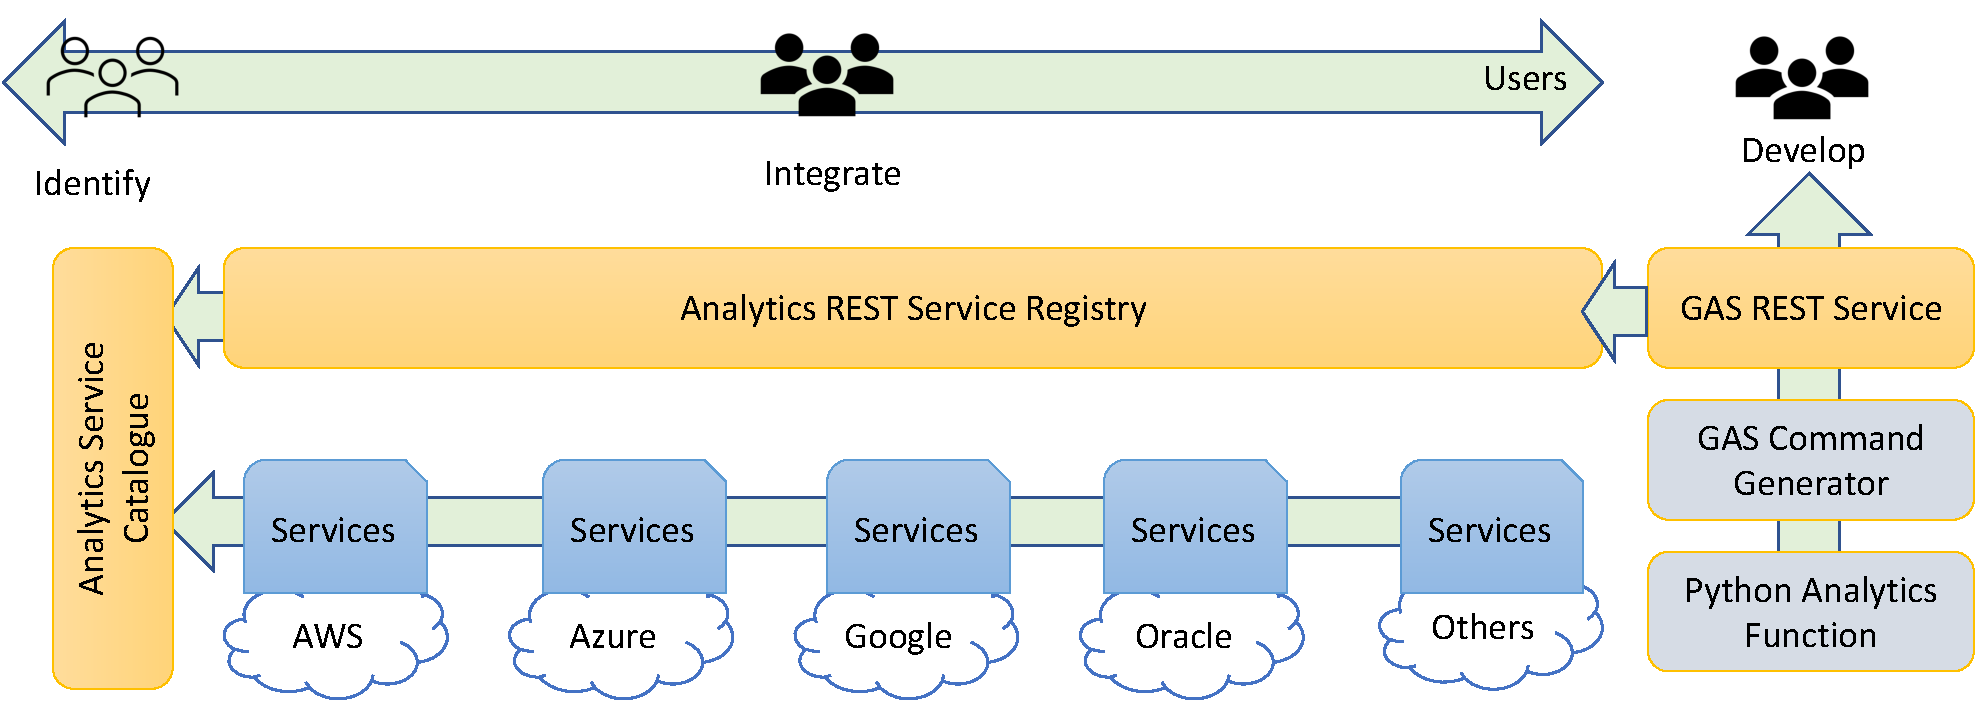
\includegraphics[width=1.0\columnwidth]{images/arch-registry.pdf}
}{This figure shows the architecture of the catalogue and registry services, as well as the possibility to create new analysis services with GAS.}
\end{center}
\vspace{-12pt}
{\em Fig 1. Layered architecture of the cloudmesh Open\-API framework.}

The reason why we need to distinguish Catalogue from Registry is based on the fact that we support with the catalogue findability without going in too much details, while the Registry provides the ability to register the details of interaction with the service, but most importantly the instantiation of such a service to encourage reusability. Furthermore our implementation of the catalouge entries is independent from a RESY specification, the registry makes explicit use of the registry. 

With this division we can first identify candidates form the plethora of services available to us and in a second step evaluate their integration details into a REST service enhanced analytics workflow. Such workflows can also be represented as high level REST services and thus become subject of reusability and deployment in larger analytics service ecosystems. 


\section*{AI Service Catalogue.}
To make it easy for users to obtain a quick overview about available AI cloud services, we have limited the initial set f attributes to those that support findability. The attributes are listed in Tab. 1. The catalogue is organized as a list of entries, where each entry contains a number of attributes. These attributes may be required or optional. 

\resizebox{0.9\columnwidth}{!}{%
\begin{tabular}{p{3cm}p{8cm}p{1cm}}
Name	& Description	& Required \\
\hline
ID	& UUID, globally unique	& \OK \\
Name	& Name of the service	& \OK \\
Title	& Human readable title 	& \OK \\
Public	& True if Public 
(needs use case to delineate what pub private means) & 	\OK \\
Description	& Human readable short Description of the Service	& \OK \\ 
Version	& The version number or tag of the service	& \OK \\
License	& The license description	& \OK \\
Microservice & 	\OK/No/Mixed	& \OK \\
Protocol	& REST	& \OK \\
Owner	& Name of the distributing entity, organization or individual. It could be a vendor.	& \OK \\
Modified	& Modification Timestamp (when first same as created)	\OK \\
Created	& Date on which the entry was first created	& \OK \\
Documentation	& Link to a URL with detailed description of the service	& O \\
Source	& Link to the source code if available	& O \\
Tag(s)	& Human readable common tags that are used to identify the service that are associated with the service	& O \\
Category(s)	& A category that this service belongs to (NLB, Finance, ...)	& O & 
Specification/ Schema	& Pointer to where schema is located &	O \\
Additional metadata	& Pointer to where additional is located including the one here.	& O \\
Endpoint	& The endpoint of the service	& O \\
SLA/Cost	&	& O \\
Authors	& contact details of the people or organization responsible for the service (freeform string)	& O \\
Data	& Description on how data is managed	& O \\
\hline
\multicolumn{3}{l}{\OK = Required; O = Optional}
\end{tabular}
}


\section*{AI Service Registry} The goal of an analytics service registry is to establish registries to locate and consume analytics services 
with persistent identifiers across organizations.  It can serve as a public, private, or federated registry. In case of a federated registry, more than one registry can be joined, to provide the user the impression of a single registry.
Within the analytics services we distinguish two classes. The first class are instantiated (running) services that are offered by a service provider and allow direct reuse. The second class are library providers that distribute analytics activity not as an instantiated service, but as a source code library which can be deployed as a service. The list of attributes are presented in Tab. 2.

\section*{Implementation.}

The implementation of the catalogue and registry are available in GitHub as open source project. It is building a basis for discussions taking place in the
NIST big data working group \cite{github-cloudmesh-catalogue}.

\resizebox{0.9\columnwidth}{!}{%
\begin{tabular}{p{3cm}p{11cm}p{0.5cm}p{0.5cm}}
Name	& Description	& \rot{\shortstack{Service\\ provider}}	& \rot{\shortstack{Library\\ provider}} \\
\hline
ID & 	UUID, globally unique &	\OK &	\OK \\
Name & 	Name of the service	& \OK	& \OK \\ 
Title & 	Human readable title &	\OK	& \OK \\
Public	& True if Public
(needs use case to delineate what pub private means) & 	\OK & \OK \\
Description	& Human readable short Description of the Service	& \OK & 	\OK \\
Endpoint &	The endpoint of the service	& \OK	&  N/A \\
List of Input Parameters &
	A list of parameters to the service. The parameters have each the form of name, function, type, value, access. The type indicates the data type. The access indicates if the parameter is a data stream, database, single value/function, event.
The function responds to a different function in case multiple are provided by the service.	& \OK	& \OK \\ 
List of Output Parameters 
  style (event, stream, data)
  value
  timestamp & 
	List of responses cast by the service. The responses have the form of function, name, type, value, access, timestamp. The type indicates the data type. The access indicates if the parameter is a data stream, database, single value/function, event.
The function responds to a different function in case multiple are provided by the service. & 	\OK 	& \OK \\
Version	& The version number or tag of the service	& \OK	& \OK \\
License	& The license description	& \OK	& \OK \\
Protocol & 	REST	& \OK	& \OK \\
Modified & 	Modification Timestamp	& \OK& \OK \\
Owner	& Name of the distributing entity, organization or individual. It could be a vendor.	& \OK	& O \\
Author &	Contact details of the people or organization responsible for the service	& O	& \OK \\
Tags &	Human readable common tags that are used to identify the service that are associated with the service	& O & O \\
Categories &	A category that this service belongs to (NLB, Finance, ...)	& O & O \\
Created	& date and time on which the analytics service was instantiated or created	instantiated	& \OK & \OK \\
Heartbeat &	State and timestamp of the last check when the service was active	& O & 	N/A \\
Documentation &	Link to a URL with detailed description of the service
Source	Link to the source code if available	& O & O \\
Specification &	Pointer to where specification schema is located	& O &  O \\
AdditionalMetadata	& Pointer to where additional is located including the one here.	& O &	O \\
SLA	& Serves level agreement including cost	& O 	& O \\
CachingInterval	&If a service is accessed a lot, the caching interval can be used to put a limitation on the Response with an LRU cache	& O &	N/A \\
DataIntegration &	In case of big data the data cannot be provided as a parameter to the analysis function. Instead, we need to provide the data as endpoint. However, often tata may need to be uploaded or can be downloaded. In this case this field provides the upload and download endpoints and the protocol to access the data	& O &	O \\
\hline
\multicolumn{3}{l}{\OK = Required; O = Optional}
\end{tabular}
}



\section*{Conclusion.}

A service registry can publicize and improve end user access to data from different sources, by overcoming some of the challenges inherent in describing and surfacing document content and format. publication, and discovery of information resources are enriched with metadata enabling the findability and reusability. While describing the interfaces and allow for the instantiation or the reuse of already instantiated services we address the accessibility and interoperability. With respect to analytics as a service, end users should be able to find various analytic services and similar services without having to individually search multiple ‘locations’ or databases, each built to operate on its own, unique storage and retrieval constructs. Through these descriptions automated service integration can be provisioned while targeting not only the functionality involved, but also allowing service level considerations to be addressed. Furthermore, such analytics services could provide significant security implications such as the protection of a database while only exposing a subset of approved analytics functions that are executed on the data sets. This includes partial and controlled sharing of data mashup that can be made available to the community and registered to make reuse easier without everyone having to replicate the service.

{\tiny
\section*{\footnotesize Acknowledgment.}

We would like to thank Lamara DeChelle Warren for initiating the contact of the UROC students so they can be part of this effort. 

\bibliographystyle{IEEEtran}
\bibliography{references}
}


\end{multicols}
\end{document}